\documentclass[aspectratio=169,10pt]{beamer}

\usetheme{metropolis}
\usepackage[main=spanish,provide=*]{babel}
\usepackage[utf8]{inputenc}
\usepackage[T1]{fontenc}
\usepackage{appendixnumberbeamer}
\usepackage{booktabs}
\usepackage{tikz}
\usepackage{forest}
\usepackage{pgfplots}
\pgfplotsset{compat=1.18}
\usetikzlibrary{positioning,calc,arrows.meta,shapes.geometric}
\usepackage{hyperref}
\usepackage{animate}

%---------- Colores corporativos UDC / FIC ----------
\definecolor{UDCmag}{RGB}{197,0,123}   % magenta UDC
\definecolor{UDCdark}{RGB}{116,10,72}  % magenta oscuro (barras de título)
\definecolor{Tcomp}{RGB}{210,224,245}  % tarea compuesta
\definecolor{Tprim}{RGB}{212,237,213}  % tarea primitiva
\definecolor{Trec}{RGB}{248,214,214}   % recuperación
\definecolor{udcpink}{RGB}{197,0,123}
\definecolor{udcgray}{RGB}{99,99,99}
\definecolor{ficblue}{RGB}{0,90,160}

\setbeamercolor{frametitle}{bg=UDCdark}
\setbeamercolor{alerted text}{fg=UDCmag}
\setbeamercolor{progress bar}{fg=UDCmag}
\setbeamercolor{title separator}{fg=UDCmag}
\setbeamercolor{palette primary}{bg=UDCdark,fg=white}
\metroset{block=fill,sectionpage=progressbar,numbering=fraction,progressbar=frametitle}

\setbeamertemplate{frame footer}{\textcolor{udcgray}{\scriptsize\insertsectionhead}}

% Atajo de resaltado
\newcommand{\hl}[1]{\textcolor{UDCmag}{\textbf{#1}}}

% Marcador para capturas / GIF / imágenes pendientes de insertar.
% Uso: \imgph{ancho}{alto}{texto}
\newcommand{\imgph}[3]{%
  \begin{tikzpicture}
    \node[draw=udcgray,dashed,line width=0.8pt,rounded corners,fill=udcgray!8,
          minimum width=#1,minimum height=#2,align=center,inner sep=4pt]
          {\footnotesize\textcolor{udcgray}{#3}};
  \end{tikzpicture}}

% Enlace a vídeo externo (YouTube / Drive): abre el navegador en CUALQUIER visor.
% Uso: \videolink{URL}{Etiqueta}
\newcommand{\videolink}[2]{%
  \begin{center}
    \href{#1}{%
      
\begin{tikzpicture}
        \node[draw=UDCmag,line width=1pt,rounded corners,fill=UDCmag!5,
              minimum width=11cm,minimum height=6.19cm] (scr) {};
        \fill[UDCmag] ([xshift=-6mm,yshift=-11mm]scr.center) --
                      ([xshift=-6mm,yshift=11mm]scr.center) --
                      ([xshift=11mm]scr.center) -- cycle;
      \end{tikzpicture}}

    {\small\href{#1}{\textcolor{UDCmag}{\underline{#2}}}\quad\textcolor{udcgray}{(abre el navegador)}}
  \end{center}%
}

%---------- Portada ----------
\title{Técnicas de inteligencia artificial\\ aplicadas en entornos simulados complejos}
\subtitle{Trabajo Fin de Grado \textbullet\ Grado en Inteligencia Artificial}
\author{Pablo Chantada Saborido}
\institute{%
  \textbf{Dirección:} Alejandro Rodríguez Arias \textbullet\ Brais Cancela Barizo\\[2pt]
  Facultade de Informática \textbullet\ Universidade da Coruña}
\date{A Coruña, 2026}
\begin{document}

\maketitle

%--------------------------------------------------------------
\begin{frame}{Guion}
  \setbeamertemplate{section in toc}[sections numbered]
  \tableofcontents[hideallsubsections]
\end{frame}

%==============================================================
\section{Minecraft como Entorno de Simulación}
%==============================================================
\begin{frame}{Qué es \textit{Minecraft}}
  \begin{columns}[T]
    \column{0.52\textwidth}
      \textit{Minecraft} es un \alert{mundo 3D hecho de bloques interactuables}.

      \vspace{0.8em}
      Lo usamos para probar agentes de IA que intenten jugar \hl{como una persona real}:
      \begin{itemize}
        \item El agente \hl{solo ve la pantalla}, como un jugador.
        \item Las acciones son \hl{muchas y encadenadas} (mirar, andar, actuar).
      \end{itemize}

    \column{0.4\textwidth}
      \centering
      \animategraphics[loop,autoplay,width=6cm]{15}{gifs/minecraft_demo}{}{}
      \vspace{0.3em}
      \mbox{\scriptsize El agente ve esta imagen, similar a un jugador humano.}
  \end{columns}
\end{frame}

%==============================================================
\section{Conceptos}
%==============================================================
\begin{frame}{Tres formas de resolver la misma tarea}
  \renewcommand{\arraystretch}{1.4}
  \centering\footnotesize
  \begin{tabular}{@{}p{2cm} p{5.6cm} p{4.4cm}@{}}    \toprule
    \textbf{Enfoque} & \textbf{Cómo decide} & \textbf{Qué necesita}\\
    \midrule
    \hl{Reglas}\newline (HTN) &
      Sigue \hl{instrucciones escritas a mano} que parten el objetivo en pasos. &
      Que un experto \hl{programe} esas reglas.\\
    \hl{Imitación}\newline (IL) &
      \hl{Copia} lo que hizo un experto. &
      \hl{Ejemplos} de un experto resolviendo la tarea.\\
    \hl{Refuerzo}\newline (RL) &
      Aprende \hl{solo}, a base de premios y castigos. &
      \hl{Muchísimos intentos} de práctica.\\
    \bottomrule
  \end{tabular}

  \vspace{0.8em}
  \footnotesize Las tres resuelven \alert{la misma tarea} para poder compararlas con justicia.
\end{frame}

%==============================================================
\section{La tarea y Arquitectura}
%==============================================================
\begin{frame}{La tarea y las reglas del juego}
  \begin{columns}[T]
    \column{0.58\textwidth}
      \textbf{Tarea común:} encontrar un árbol, acercarse y \hl{recoger 5 troncos}.
      Es el primer paso de la progresión del juego.

      \vspace{0.5em}
      \textbf{Percepción:} el agente \hl{solo ve lo que vería un jugador humano} en la
      pantalla. No sabe dónde están las cosas; tiene que \hl{mirarlas directamente} para
      encontrarlas.

      \vspace{0.5em}
      \textbf{Misma prueba:} mismo mundo, mismo punto de partida y la misma forma de medir
      el éxito para los tres enfoques.
    \column{0.42\textwidth}
      \centering
      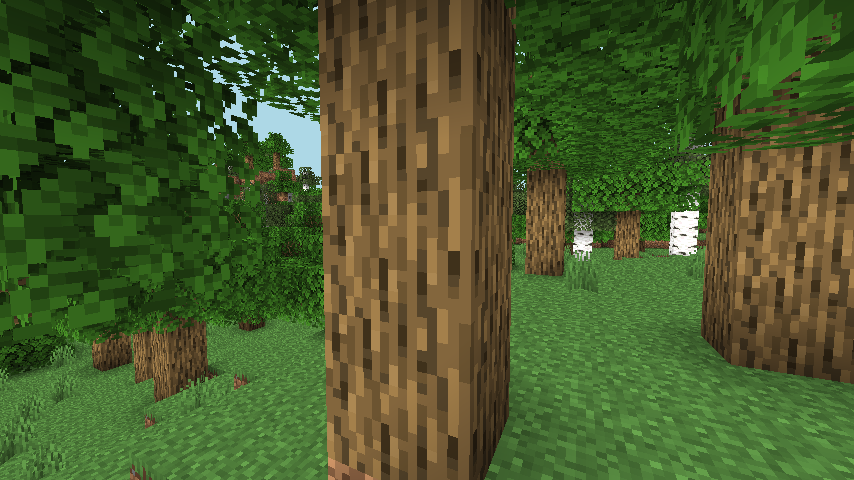
\includegraphics[width=\linewidth]{imaxes/anexos/imagen_visor.png}

      \vspace{0.3em}
      \mbox{\scriptsize El agente recibe una imagen y un vector de estado.}
  \end{columns}
\end{frame}

\begin{frame}{Un mismo sistema para los tres enfoques}
  \centering
  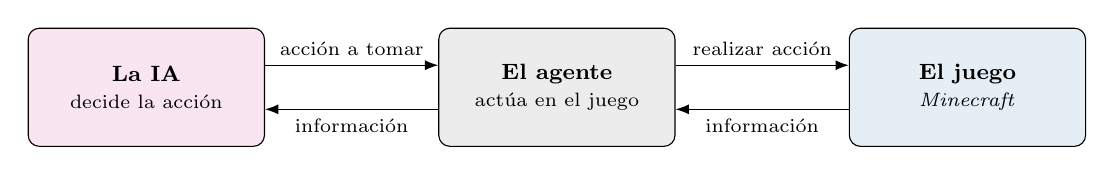
\begin{tikzpicture}[font=\footnotesize,>=Latex,
      box/.style={draw,rounded corners,align=center,minimum width=30mm,minimum height=15mm}]
    \node[box,fill=UDCmag!10] (ia) {\textbf{La IA}\\\scriptsize decide la acción};
    \node[box,fill=udcgray!12,right=22mm of ia] (ag) {\textbf{El agente}\\\scriptsize actúa en el juego};
    \node[box,fill=ficblue!10,right=22mm of ag] (game) {\textbf{El juego}\\\scriptsize\textit{Minecraft}};
    \draw[->] ([yshift=2.8mm]ia.east) -- node[above,font=\scriptsize]{acción a tomar} ([yshift=2.8mm]ag.west);
    \draw[<-] ([yshift=-2.8mm]ia.east) -- node[below,font=\scriptsize]{información} ([yshift=-2.8mm]ag.west);
    \draw[->] ([yshift=2.8mm]ag.east) -- node[above,font=\scriptsize]{realizar acción} ([yshift=2.8mm]game.west);
    \draw[<-] ([yshift=-2.8mm]ag.east) -- node[below,font=\scriptsize]{información} ([yshift=-2.8mm]game.west);
  \end{tikzpicture}

  \vspace{1em}
  El algoritmo de \hl{IA} indica \hl{qué acción} debe realizar el agente; este la ejecuta sobre el entorno y obtiene una \hl{observación}, sobre la que toma la \hl{siguiente decisión}.

  \vspace{0.3em}
  \alert{Es el mismo montaje para los tres enfoques}, comparten la obtención de la información y la ejecución de las acciones.
\end{frame}

%==============================================================
\section{Iteración I: HTN}
%==============================================================
\begin{frame}{Reglas: partir el objetivo en pasos sencillos}
  \begin{columns}[T]
    \column{0.56\textwidth}
      \centering
      \begin{forest}
        for tree={font=\scriptsize, grow'=0, draw, rounded corners, inner sep=2.5pt,
          parent anchor=south, child anchor=west, anchor=west, calign=first,
          edge={semithick}, l sep=4mm, s sep=1mm,
          edge path={\noexpand\path[draw,\forestoption{edge}]
            (!u.south west)+(6pt,0) |- (.child anchor)\forestoption{edge label};},
          before typesetting nodes={if n=1{insert before={[,phantom]}}{}},
          fit=band, before computing xy={l=14pt}}
        [Recoger 5 troncos,fill=Tcomp
          [Elegir un árbol,fill=Tprim]
          [Talar un árbol (repetir),fill=Tcomp
            [Buscar un árbol a la vista,fill=Tprim]
            [Explorar si no hay ninguno,fill=Trec]
            [Ir hasta el árbol,fill=Tprim]
            [Talarlo entero,fill=Tcomp
              [Romper la base,fill=Tprim]
              [Subir y talar el resto,fill=Tprim]
            ]
          ]
        ]
      \end{forest}
    \column{0.44\textwidth}
      \footnotesize
      Un experto del dominio escribe \hl{a mano} la lista de pasos y cuándo aplicar cada uno.

      \vspace{0.6em}
      \begin{tabular}{@{}l@{\hspace{1.5mm}}l@{}}
        \tikz\fill[Tcomp](0,0) rectangle (0.30,0.30); & Tarea Compuesta (se divide en otras)\\[2pt]
        \tikz\fill[Tprim](0,0) rectangle (0.30,0.30); & Tarea Primitiva (acción directa)\\[2pt]
        \tikz\fill[Trec](0,0) rectangle (0.30,0.30);  & Tarea Recuperación (si algo falla)\\
      \end{tabular}

      \vspace{0.8em}
      \textbf{Si un paso falla}, prueba una alternativa o explora antes de reintentar.

      \vspace{0.8em}
      \begin{alertblock}{Doble papel}
        Sirve de \hl{referencia} y, además, genera los \hl{ejemplos} para el enfoque por imitación.
      \end{alertblock}
  \end{columns}
\end{frame}

\begin{frame}{Reglas: funciona siempre... pero con ventaja}
  \begin{columns}[T]
    \column{0.46\textwidth}
      \textbf{Resultados (50 partidas)}
      \vspace{0.3em}
      \begin{table}\centering\small
        \begin{tabular}{@{}lc@{}}
          \toprule
          Tasa de éxito & \hl{100\,\%}\\
          Troncos recolectados & 6.0\\
          Tiempo por partida & 27 s\\
          \bottomrule
        \end{tabular}
      \end{table}
      \vspace{0.4em}
      \footnotesize Siempre lo consigue y muy rápido, sin necesidad de entrenar.

      \vspace{0.6em}
      \begin{alertblock}{Por qué acierta el 100\,\%}
        \footnotesize Porque "hace trampas": usa \hl{datos exactos} del juego (dónde está
        cada cosa) que los demás agentes \hl{no} tienen.
      \end{alertblock}

    \column{0.54\textwidth}
      \centering
      \animategraphics[loop,autoplay,width=6.4cm]{15}{gifs/htn_native}{}{}
      \vspace{0.3em}
      {\scriptsize Ejecución del agente HTN.}
  \end{columns}

  \vspace{0.5em}
  \footnotesize
  Pero depende de reglas \hl{escritas a mano}, y para tareas más complejas escribirlas todas
  \alert{se vuelve inviable} $\Rightarrow$ por eso medimos también a los que aprenden
  \hl{solo mirando la pantalla}.
\end{frame}

%==============================================================
\section{Iteración II: IL}
%==============================================================
\begin{frame}{Imitación: aprender copiando al experto}
  \centering
  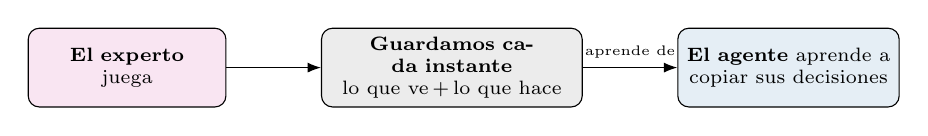
\begin{tikzpicture}[font=\scriptsize,>=Latex,
      b/.style={draw,rounded corners,align=center,minimum height=10mm,inner sep=3pt}]
    \node[b,fill=UDCmag!10,text width=2.3cm] (exp) {\textbf{El experto}\\ juega};
    \node[b,fill=udcgray!12,text width=3.1cm,right=12mm of exp] (dat)
      {\textbf{Guardamos cada instante}\\lo que ve\,+\,lo que hace};
    \node[b,fill=ficblue!10,text width=2.6cm,right=12mm of dat] (ia)
      {\textbf{El agente} aprende a\\copiar sus decisiones};
    \draw[->] (exp) -- (dat);
    \draw[->] (dat) -- node[above,font=\tiny]{aprende de} (ia);
  \end{tikzpicture}

  \vspace{0.5em}
  \begin{columns}[T]
    \column{0.46\textwidth}
      \footnotesize
      \textbf{Los datos del experto}
      \begin{itemize}\footnotesize\itemsep2pt
        \item \hl{118 partidas}.
        \item De cada instante: \hl{lo que veía} (imagen) y \hl{lo que hizo} (acción).
      \end{itemize}
      \vspace{0.2em}
      \textbf{La dificultad}
      \begin{itemize}\footnotesize\itemsep2pt
        \item El experto \hl{repite mucho una sola acción} (talar), así que el agente
        tiende a \hl{copiar solo esa}: hubo que reequilibrar los datos.
      \end{itemize}
    \column{0.54\textwidth}
      \centering
      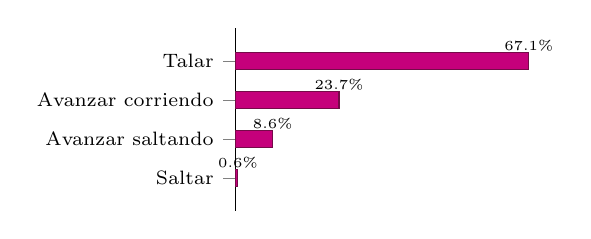
\begin{tikzpicture}
        \begin{axis}[
          xbar, width=6.4cm, height=3.9cm, bar width=6pt,
          xmin=0, xmax=3550, clip=false,
          symbolic y coords={Saltar,{Avanzar saltando},{Avanzar corriendo},Talar},
          ytick=data, y tick label style={font=\scriptsize},
          axis x line=none, axis y line*=left, tick align=outside,
          enlarge y limits=0.28, nodes near coords, nodes near coords style={font=\tiny},
          point meta=explicit symbolic]
          \addplot[fill=UDCmag,draw=UDCdark] coordinates {
            (25,Saltar)[0.6\%]
            (351,{Avanzar saltando})[8.6\%]
            (971,{Avanzar corriendo})[23.7\%]
            (2747,Talar)[67.1\%]};
        \end{axis}
      \end{tikzpicture}

      {\scriptsize El experto usa muy pocas acciones: los datos están \hl{desequilibrados}.}
  \end{columns}
\end{frame}

\begin{frame}{Imitación: cómo aprende de las imágenes}
  \begin{columns}[T]
    \column{0.52\textwidth}
      \centering
      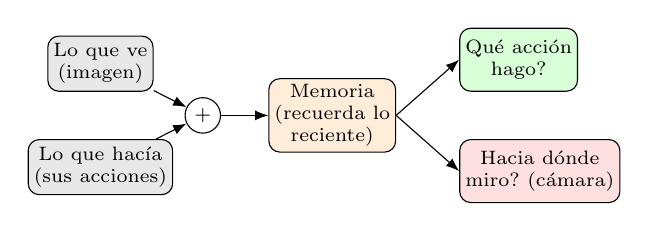
\begin{tikzpicture}[font=\scriptsize,>=Latex,node distance=5mm,
          io/.style ={draw,rounded corners,fill=udcgray!15,align=center,minimum height=7mm,inner sep=2pt},
          mem/.style={draw,rounded corners,fill=orange!15,align=center,minimum height=9mm,inner sep=2pt},
          hc/.style ={draw,rounded corners,fill=green!15,align=center,minimum height=8mm,inner sep=2pt},
          hr/.style ={draw,rounded corners,fill=red!12,align=center,minimum height=8mm,inner sep=2pt},
          sum/.style={draw,circle,inner sep=1pt,minimum size=4.5mm}]
        \node[io] (img) {Lo que ve\\(imagen)};
        \node[io] (st) [below=6mm of img] {Lo que hacía\\(sus acciones)};
        \node[sum] (s) at ($(img)!0.5!(st)+(13mm,0)$) {$+$};
        \node[mem] (m) [right=6mm of s] {Memoria\\\scriptsize(recuerda lo\\\scriptsize reciente)};
        \node[hc] (ah) [above right=3mm and 8mm of m.east] {Qué acción\\hago?};
        \node[hr] (ch) [below right=3mm and 8mm of m.east] {Hacia dónde\\miro? (cámara)};
        \draw[->] (img) -- (s);
        \draw[->] (st) -- (s);
        \draw[->] (s) -- (m);
        \draw[->] (m.east) -- (ah.west);
        \draw[->] (m.east) -- (ch.west);
      \end{tikzpicture}

      \vspace{0.4em}
      {\scriptsize Mira cada imagen y responde con la acción que habría hecho el experto.}
    \column{0.48\textwidth}
      \footnotesize
      \begin{itemize}\itemsep6pt
        \item Probamos \hl{varias redes distintas} para ver si el agente aprende más de
        \hl{la imagen} o de \hl{la secuencia de sus acciones recientes}.
        \item \hl{Mejora clave:} separar \alert{hacia dónde mira} (la cámara) del resto de
        acciones. Al dejar de estorbarse entre sí, el agente mejoró.
        \item \hl{Sin la imagen, apenas se mueve}: ver la pantalla es lo que le permite actuar.
      \end{itemize}
  \end{columns}
\end{frame}

\begin{frame}{Imitación: qué redes probamos}
  Todas copian al experto; lo que cambia es \hl{cómo procesan la imagen}:
  \begin{itemize}\itemsep5pt
    \item \hl{GRU}: lee la imagen \hl{por franjas}, de arriba abajo, y
    va \hl{recordando} lo que ve.
    \item \hl{ConvLSTM}: combina \hl{visión} con \hl{memoria} de lo más reciente.
    \item \hl{ViT}: una red visual \hl{ya entrenada con millones de imágenes}, adaptada a
    nuestra tarea.
    \item \hl{Solo estado}: \hl{sin mirar la imagen}, como referencia para medir cuánto
    aporta ver.
  \end{itemize}

  \vspace{0.4em}
  \begin{alertblock}{Lo que encontramos}
    La \hl{GRU} fue la que mejor imitó al experto, y \hl{todas las que ven la imagen}
    superan a la que \hl{no la ve}.
  \end{alertblock}
\end{frame}

\begin{frame}{Imitación: aprende a talar, pero no a buscar}
  \begin{columns}[T]
    \column{0.46\textwidth}
      \textbf{Tasa de éxito}
      \begin{table}\centering\small
        \begin{tabular}{@{}lc@{}}
          \toprule
          \hl{GRU (mejor)} & \hl{52\,\%}\\
          ViT & 46\,\%\\
          Sin imagen & 4\,\%\\
          \bottomrule
        \end{tabular}
      \end{table}
      \footnotesize Lo mejor entre los agentes que \emph{aprenden}.

      \vspace{0.6em}
      \begin{alertblock}{El límite de imitar}
        \footnotesize Aprende a talar un árbol que \hl{ya tiene delante},
        pero \hl{no a buscarlo}.
      \end{alertblock}

    \column{0.54\textwidth}
      \centering
      \animategraphics[loop,autoplay,width=6.4cm]{15}{gifs/gru}{}{}
      \vspace{0.3em}
      {\scriptsize Ejecución del agente de imitación.}
  \end{columns}

  \vspace{0.5em}
  \footnotesize
  El experto iba siempre directo al árbol, así que en los ejemplos \alert{nunca aparece la
  fase de buscar}. Si el agente se desvía, llega a situaciones que nunca vio y
  \hl{los errores se acumulan} $\Rightarrow$ esto motiva el siguiente enfoque:
  \textbf{Aprendizaje por Refuerzo}.
\end{frame}

%==============================================================
\section{Iteración III: RL}
%==============================================================
\begin{frame}{Refuerzo: aprender solo, con premios y castigos}
  \begin{columns}[T]
    \column{0.54\textwidth}
      El agente \hl{no tiene ejemplos ni reglas}. Practica una y otra vez y aprende de las
      consecuencias: lo que le acerca al objetivo le da \hl{premio}; lo que no, \hl{castigo}.

      \vspace{0.6em}
      Probamos \hl{tres formas distintas} de aprender así:
      \begin{itemize}\itemsep4pt\footnotesize
        \item \hl{DQN}: estima "cómo de buena" es cada acción y elige la mejor.
        \item \hl{PPO}: ajusta su forma de jugar \hl{poco a poco}, sin cambios bruscos.
        \item \hl{SAC}: busca el premio sin dejar de \hl{probar cosas nuevas}.
      \end{itemize}
    \column{0.46\textwidth}
      \centering
      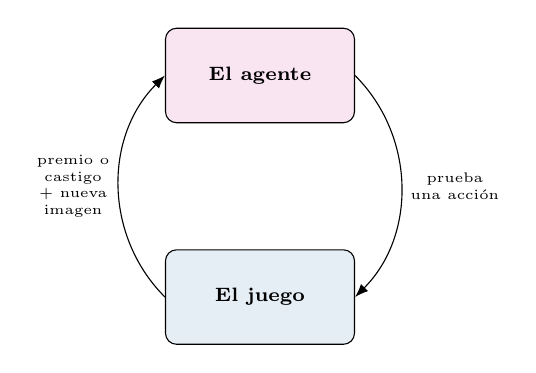
\begin{tikzpicture}[font=\scriptsize,>=Latex,
          b/.style={draw,rounded corners,align=center,minimum width=24mm,minimum height=12mm}]
        \node[b,fill=UDCmag!10] (ag) {\textbf{El agente}};
        \node[b,fill=ficblue!10,below=16mm of ag] (env) {\textbf{El juego}};
        \draw[->] (ag.east) to[bend left=45] node[right,align=center,font=\tiny]{prueba\\una acción} (env.east);
        \draw[->] (env.west) to[bend left=45] node[left,align=center,font=\tiny]{premio o\\castigo\\+ nueva\\imagen} (ag.west);
      \end{tikzpicture}

      \vspace{0.2em}
      {\scriptsize Prueba, mira el resultado y ajusta.}
  \end{columns}
\end{frame}

\begin{frame}{Refuerzo: cómo premiamos al agente}
  \centering
  {\small Sumamos premios y restamos castigos en cada partida:}

  \vspace{0.4em}
  \renewcommand{\arraystretch}{1.15}
  \footnotesize
  \begin{tabular}{@{}lcl@{}}
    \toprule
    \textbf{Qué pasa} & \textbf{Valor} & \textbf{Para qué}\\
    \midrule
    Completa la tarea       & \hl{$+30$}  & Gran recompensa final\\
    Rompe un tronco         & \hl{$+20$}  & Objetivo principal\\
    Recoge un tronco        & $+5$        & Buen estado\\
    \addlinespace[2pt]
    Golpea un árbol         & $+1$        & Estado correcto\\
    Se acerca a un árbol    & $+0.1$      & Estado correcto\\
    \addlinespace[2pt]
    Cada paso que da        & $-0.05$     & Eficiencia\\
    Golpea algo que no toca & $-1$        & Evitar errores\\
    Muere o se acaba el tiempo & $-5$     & Castigo por fallar\\
    \bottomrule
  \end{tabular}

  \vspace{0.6em}
  \footnotesize Usamos \hl{recompensas intermedias}: sin ellas, el premio llegaría tan tarde que no aprendería.
\end{frame}

\begin{frame}{Refuerzo: un ganador claro, pero le falta práctica}
  \begin{columns}[T]
    \column{0.44\textwidth}
      \textbf{Tasa de éxito}
      \begin{table}\centering\small
        \begin{tabular}{@{}lc@{}}
          \toprule
          \hl{PPO} & \hl{12\,\%}\\
          Al azar & 6\,\%\\
          SAC & 4\,\%\\
          DQN & 2\,\%\\
          \bottomrule
        \end{tabular}
      \end{table}
      \footnotesize Solo \hl{PPO} supera al azar: se centra en lo productivo (avanzar y
      talar), como el experto; los demás exploran mal y se quedan cerca del azar.
    \column{0.56\textwidth}
      \centering
      \animategraphics[loop,autoplay,width=5.9cm]{15}{gifs/rl_native}{}{}
      \vspace{0.2em}
      \mbox{\scriptsize Ejecución del agente de refuerzo.}
  \end{columns}

  \vspace{0.1em}
  \begin{alertblock}{El cuello de botella: tiempo de cómputo}
    \footnotesize Otros trabajos entrenan con \hl{$\sim$1500 partidas} (aquí serían meses por
    algoritmo); nosotros pudimos hacer \hl{$\sim$200} ($\approx$2 h).
    \hl{Sí aprende; lo que falta es iterar.}
  \end{alertblock}
\end{frame}

%==============================================================
\section{Resultados y conclusiones}
%==============================================================
\begin{frame}{Comparativa global}
  \centering
  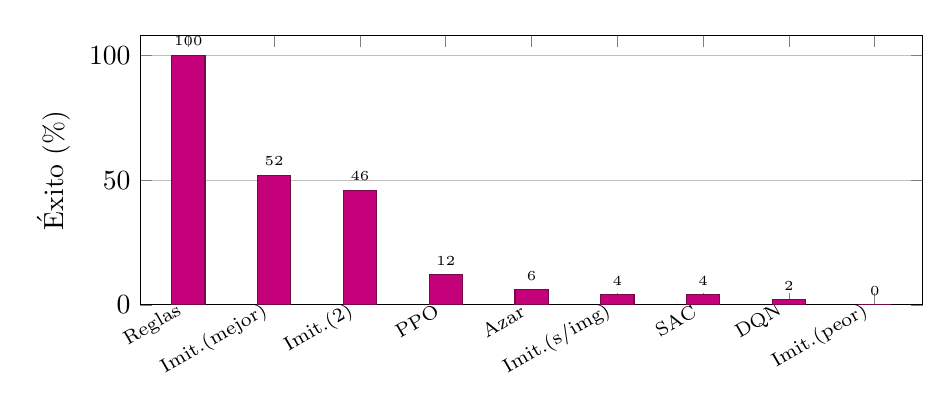
\begin{tikzpicture}
    \begin{axis}[
      ybar, width=0.95\linewidth, height=5.0cm, bar width=12pt,
      ymin=0, ymax=108, ylabel={Éxito (\%)},
      symbolic x coords={Reglas,Imit.(mejor),Imit.(2),PPO,Azar,Imit.(s/img),SAC,DQN,Imit.(peor)},
      xtick=data, x tick label style={rotate=30,anchor=east,font=\scriptsize},
      nodes near coords, nodes near coords style={font=\tiny},
      enlarge x limits=0.07, ymajorgrids, tick align=inside]
      \addplot[fill=UDCmag,draw=UDCdark] coordinates
        {(Reglas,100)(Imit.(mejor),52)(Imit.(2),46)(PPO,12)(Azar,6)(Imit.(s/img),4)(SAC,4)(DQN,2)(Imit.(peor),0)};
    \end{axis}
  \end{tikzpicture}

  \vspace{0.3em}
  \alert{Reglas (100\%) $\gg$ Imitación ($\sim$50\%) $\gg$ Refuerzo (12\%) $>$ azar}

  \vspace{0.2em}
  \footnotesize El \hl{conocimiento del experto} y el \hl{uso de la imagen} obtienen los mejores resultados.
\end{frame}

\begin{frame}{Comparativa: \textquestiondown y si pedimos menos troncos?}
  \centering
  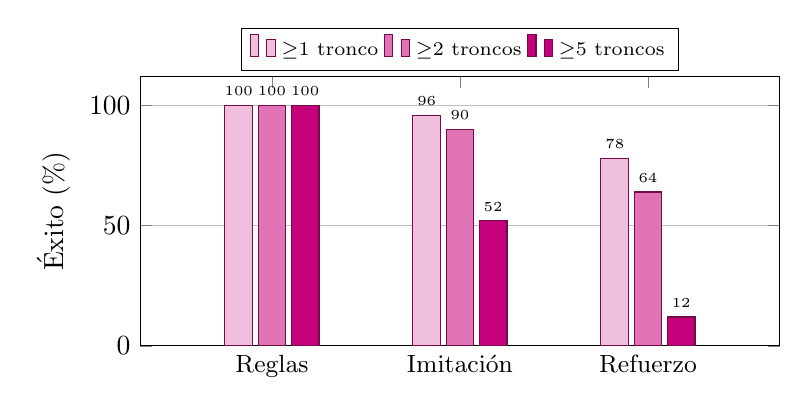
\begin{tikzpicture}
    \begin{axis}[
      ybar, width=0.8\linewidth, height=5.0cm, bar width=10pt,
      ymin=0, ymax=112, ylabel={Éxito (\%)},
      symbolic x coords={Reglas,Imitación,Refuerzo}, xtick=data,
      x tick label style={font=\small},
      nodes near coords, nodes near coords style={font=\tiny},
      enlarge x limits=0.35, ymajorgrids, tick align=inside,
      legend style={font=\scriptsize,at={(0.5,1.02)},anchor=south,legend columns=3}]
      \addplot[fill=UDCmag!25,draw=UDCdark] coordinates {(Reglas,100)(Imitación,96)(Refuerzo,78)};
      \addplot[fill=UDCmag!55,draw=UDCdark] coordinates {(Reglas,100)(Imitación,90)(Refuerzo,64)};
      \addplot[fill=UDCmag,draw=UDCdark]    coordinates {(Reglas,100)(Imitación,52)(Refuerzo,12)};
      \legend{$\geq$1 tronco,$\geq$2 troncos,$\geq$5 troncos}
    \end{axis}
  \end{tikzpicture}

  \vspace{0.3em}
  \footnotesize Al reducir la dificultad de la tarea todos mejoran, pero \hl{el orden se mantiene}: refleja lo que cada técnica ha aprendido de verdad.
\end{frame}

\begin{frame}{Tabla de resultados (recoger 5 troncos)}
  \centering\footnotesize
  \renewcommand{\arraystretch}{1.05}
  \resizebox{\textwidth}{!}{%
  \begin{tabular}{@{}llc c ccc ccc@{}}
    \toprule
    & & & & \multicolumn{3}{c}{\textbf{Troncos}} & \multicolumn{3}{c}{\textbf{Tiempo (s)}}\\
    \cmidrule(lr){5-7}\cmidrule(lr){8-10}
    \textbf{Enfoque} & \textbf{Variante} & \textbf{Part.} & \textbf{Éxito (\%)}
      & $\mu$ & $\tilde{x}$ & $\sigma$ & $\mu$ & $\tilde{x}$ & $\sigma$\\
    \midrule
    Reglas     & \hl{HTN}         & 50 & \hl{100.0} & 6.00 & 6.00 & 0.00 & 26.7  & 26.4  & 1.1\\
    \midrule
    Imitación  & \hl{Mejor (GRU)} & 50 & \hl{52.0}  & 3.84 & 5.00 & 1.82 & 156.2 & 203.4 & 67.3\\
               & Variante 2       & 50 & 46.0       & 3.48 & 5.00 & 1.82 & 156.7 & 206.1 & 70.9\\
               & Sin imagen       & 50 & 4.0        & 0.54 & 0.00 & 1.25 & 195.8 & 202.1 & 34.1\\
               & Peor             & 50 & 0.0        & 0.08 & 0.00 & 0.27 & 203.0 & 202.1 & 3.3\\
    \midrule
    Refuerzo   & \hl{PPO}         & 50 & \hl{12.0}  & 2.14 & 2.00 & 1.64 & 114.6 & 124.5 & 43.3\\
               & Al azar          & 50 & 6.0        & 1.50 & 1.00 & 1.52 & 97.6  & 111.1 & 40.3\\
               & SAC              & 50 & 4.0        & 1.62 & 1.00 & 1.41 & 110.6 & 114.3 & 31.3\\
               & DQN              & 50 & 2.0        & 1.10 & 0.00 & 1.40 & 117.6 & 121.5 & 28.8\\
    \bottomrule
  \end{tabular}}

  \vspace{0.3em}
  {\scriptsize $\mu$ = media, $\tilde{x}$ = mediana, $\sigma$ = variabilidad entre partidas.}
\end{frame}

\begin{frame}{Conclusiones}
  Nuestra principal aportación es \hl{un banco de pruebas justo} para comparar los tres
  enfoques sin que ninguno parta con ventaja:
  \begin{itemize}\itemsep6pt
    \item \hl{Misma tarea y mismas condiciones:} idéntico mundo, punto de partida y forma de
    medir el éxito, así ninguna diferencia viene del montaje.
    \item \hl{Misma percepción:} todos \hl{ven lo mismo} (salvo las reglas, que lo hacen
    explícito como límite superior), no datos privilegiados unos sí y otros no.
    \item \hl{Datos y tutor propios:} los ejemplos del experto los generamos nosotros con las
    reglas, que sirven a la vez de \hl{referencia} y de \hl{fuente de datos} para imitación.
  \end{itemize}

  \vspace{0.6em}
  \begin{alertblock}{La lección de la comparativa}
    \footnotesize Sobre esa base justa, el orden es claro: aprovechar el \hl{conocimiento del
    experto} (reglas e imitación) rinde mucho más que \hl{aprender desde cero} (refuerzo), que
    apenas empieza a despegar con el cómputo disponible.
  \end{alertblock}
\end{frame}

\begin{frame}{Trabajo futuro}
  \begin{itemize}\itemsep6pt
    \item \hl{Combinar enfoques:} usar las reglas como \hl{guía} para el agente de refuerzo,
    para enseñarle a explorar.
    \item \hl{Mejorar la imitación:} más ejemplos y otras redes neuronales.
    \item \hl{Tareas más difíciles:} usar este mismo sistema para retos mayores
    (conseguir hierro, diamante, construir).
  \end{itemize}
\end{frame}

%-------------------- CIERRE --------------------
\begin{frame}[standout]
  \textexclamdown Gracias!\\[0.4em]
  {\normalsize \textquestiondown Preguntas?}
\end{frame}

%==============================================================
\appendix
%==============================================================
\begin{frame}{Arquitectura del sistema}
  \centering
  \resizebox{\textwidth}{!}{%
  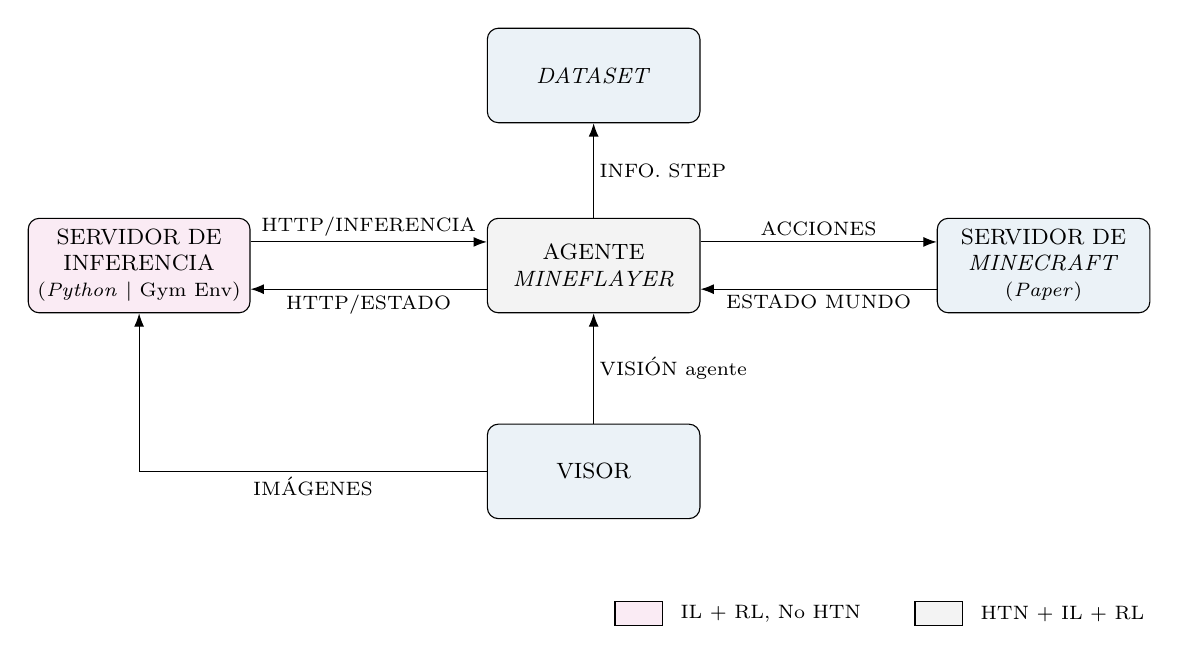
\begin{tikzpicture}[
    font=\footnotesize, >=Latex,
    box/.style={draw, rounded corners, align=center, minimum width=27mm, minimum height=12mm},
    lbl/.style={font=\scriptsize, align=center, inner sep=2pt},
    legbox/.style={draw, minimum width=6mm, minimum height=3mm, inner sep=0pt}
  ]
    \node[box, fill=udcpink!8]  (serv)  {SERVIDOR DE\\INFERENCIA\\{\scriptsize(\textit{Python} \textbar{} Gym Env)}};
    \node[box, fill=udcgray!8]  (ag)    [right=30mm of serv] {AGENTE\\\textit{MINEFLAYER}};
    \node[box, fill=ficblue!8]  (mc)    [right=30mm of ag]   {SERVIDOR DE\\\textit{MINECRAFT}\\{\scriptsize(\textit{Paper})}};
    \node[box, fill=ficblue!8]  (data)  [above=12mm of ag]   {\textit{DATASET}};
    \node[box, fill=ficblue!8]  (visor) [below=14mm of ag]   {VISOR};

    % Servidor de inferencia <-> Agente
    \draw[->] ([yshift=3mm]serv.east) -- node[lbl,above]{HTTP/INFERENCIA} ([yshift=3mm]ag.west);
    \draw[->] ([yshift=-3mm]ag.west)  -- node[lbl,below]{HTTP/ESTADO}     ([yshift=-3mm]serv.east);
    % Agente -> Dataset
    \draw[->] (ag) -- node[lbl,right]{INFO.\ STEP} (data);
    % Agente <-> Servidor de Minecraft
    \draw[->] ([yshift=3mm]ag.east)  -- node[lbl,above]{ACCIONES}     ([yshift=3mm]mc.west);
    \draw[->] ([yshift=-3mm]mc.west) -- node[lbl,below]{ESTADO MUNDO} ([yshift=-3mm]ag.east);
    % Visor -> Agente
    \draw[->] (visor) -- node[lbl,right]{VISIÓN agente} (ag);
    % Visor -> Servidor (entrada visual)
    \draw[->] (visor.west) -| node[lbl,below,pos=0.25]{IMÁGENES} (serv.south);

    % --- LEYENDA (Abajo a la derecha) ---
    \coordinate (legend_pos) at ($(mc.east |- visor.south) + (0,-12mm)$);
    \node[lbl, anchor=east] (ljs_text) at (legend_pos) {HTN + IL + RL};
    \node[legbox, fill=udcgray!8, left=1.5mm of ljs_text, anchor=east] (ljs) {};

    \node[lbl, left=6mm of ljs, anchor=east] (lpy_text) {IL + RL, No HTN};
    \node[legbox, fill=udcpink!8, left=1.5mm of lpy_text, anchor=east] (lpy) {};
  \end{tikzpicture}}

  \vspace{0.6em}
  \footnotesize La \hl{capa de decisión} (\textit{Python}) se comunica por \hl{HTTP} con el agente
  (\textit{Mineflayer}), que actúa sobre el \hl{servidor de Minecraft}; las reglas (\hl{HTN})
  viven por completo en el agente.
\end{frame}

\end{document}